\chapter{System Analysis}
Project details and descriptions of modules are in this section.
This project will contains a mobile application which saves user location, media files and organize an event with other people, and a server side application which provides users to interact, sharing saved contents and access shared contents. 

Mobile application will saved location, notes and media files also location of media files to storage when user started trip tracking feature of mobile application. Before starting a trip user can choose some of his/her friends to organize a trip with them on the both online and offline modes. If searching friend is not listed on offline mode, user can add friend when internet connection provided. If a person added a trip, this person will give a notification which asks user to accept joining or reject joining to trip. If user accepted invitation he/she can join trip as a member. Invitor is accepted as leader of team. During the trip all user's behavior saved seperately. If location sharing feature opened any member of this team can watch other members location. But as we mentioned this feature requires internet connection. At the end of trip when user want to share his/her trip data and all of the data shared by other members will be merged. All users can select sharing data seperately. As a result anyone could wants to store a picture but don't want to share. 

In order to save location on background Android application will use a location saving service. Using service is a must because, Android services provides to execute a process for long time on the background. User can watch his/her location path on map during trip. If user wants to track a path which is shared from other people user can track the path by looking at map.

Modules created by project team as follows:
\begin{itemize}
    \item User register module
    \item User login module
    \item Trip search module
    \item Location save module
    \item Media save module
    \item Feature extraction module
    \item Trip management module
    \item Notification sender module
    \item Trip upload module
    \item Trip download module
    \item Team content merging module
\end{itemize}

\section{Modules}

\subsection{User Register Module}
User register module provides creating new users. This module needs user name, password and email from user to create a new account. This module runs on web application but user can use this module on mobile and web application.
\subsection{User Login Module}
User login module provides user to sing in into mobile and web application. This module needs user name and password from user to sing in. This module runs on web application but user can use this module on mobile and web application.
\subsection{Trip Seach Module}
This module provides user to search shared trips by region, user, time and trip type. User can only search on trips which he/she have permission to see. This module runs on web application but user can use this module on mobile and web application. 
\subsection{Location Save Module}
This module runs as a background task on Android device and saves navigation(longitude, latitude, altitude) data provided from GPS to a CSV file. This module runs on mobile application.
\subsection{Media Save Module}
This module saves photo, video and sound record with their location data to SQLite database on Android device. This module runs on mobile application.
\subsection{Feature Extraction Module}
This module tags trips using trip path data by their country, province, distinct, members, time and trip type on the web application. This module runs on web application.
\subsection{Trip Management Module}
This module provides user to add new members to trip or manage trip contents like deleting a photo or changing access privileges for contents. This module runs on mobile application.
\subsection{Notification Sender Module}   
This module provides sending notifications to users about any topic. This module runs on web application but mobile application use this module as a web service.
\subsection{Trip Upload Module}
This module provides user to share trip content on social media with determined access rights. Mobile application prepares a zip file which includes all of chosen contents belong to trip and upload this zip file to server side using web application.
\subsection{Trip Download Module}
This module provides user to download chosen contents of a trip which he/she has access rights to his/her mobile device. Web application prepares a zip file using choosen contents and send it to mobile application.
\subsection{Team Content Merging Module}
This module provides trip members to merge trip content easily for share on social media. Web application merges all of sended contents from members in one trip.

\newpage 
\section{UML and Database Diagrams}

\begin{figure}[!htbp]
\centering
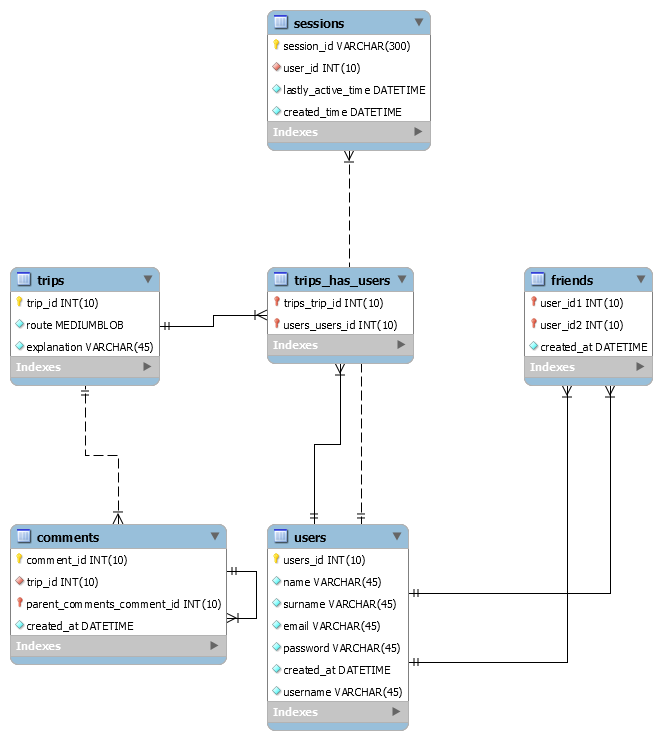
\includegraphics[width=\textwidth]{projectChapters/images/databaseDesign.png}
\caption{Backend Database design pattern}
\end{figure}
 
 
\begin{figure}[!htbp]
\centering
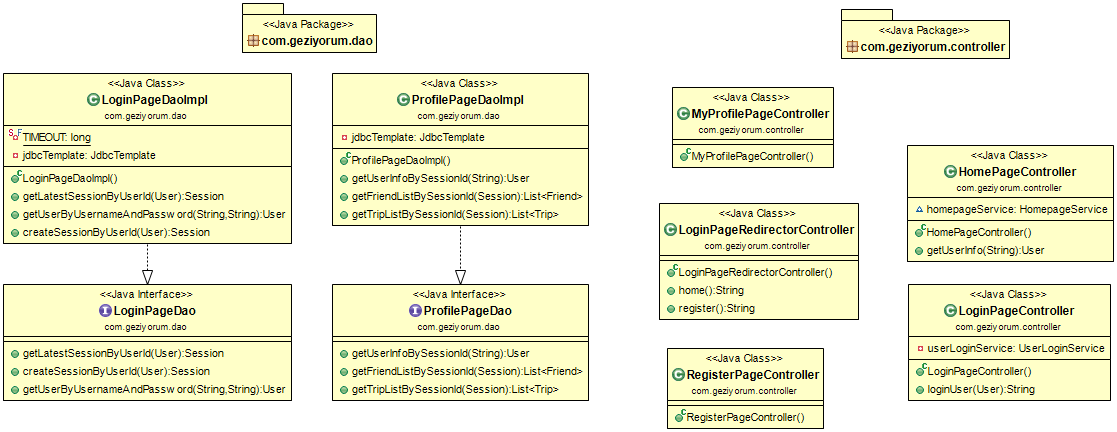
\includegraphics[width=\textwidth]{projectChapters/images/backend1.png}
\caption{Backend implementation MVC UML-1}
\end{figure}

\begin{figure}[!htbp]
\centering
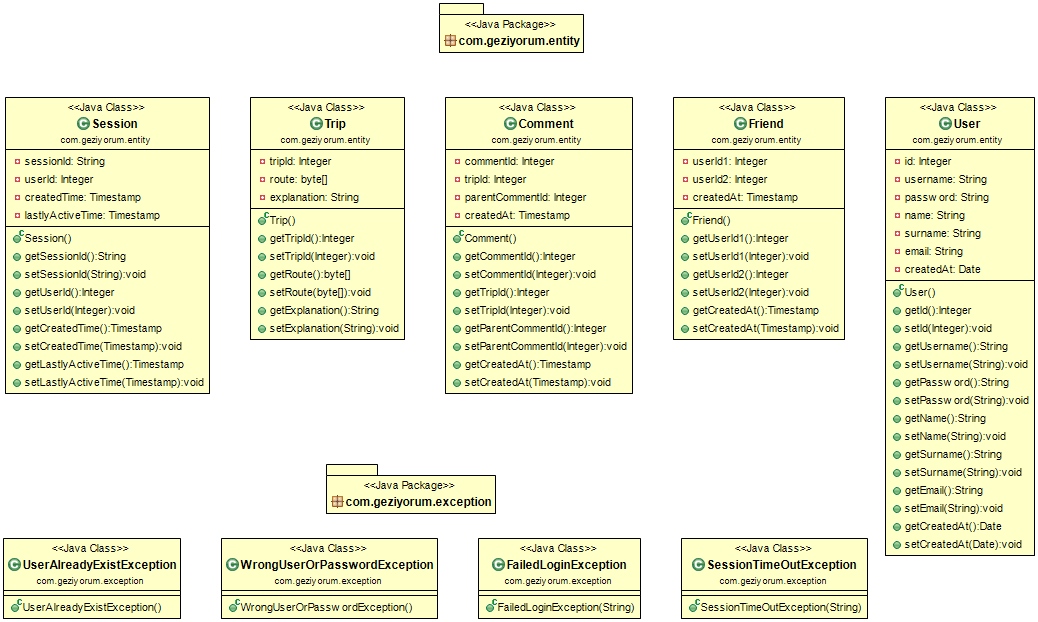
\includegraphics[width=\textwidth]{projectChapters/images/backend2.png}
\caption{Backend implementation MVC UML-2}
\end{figure}


\begin{figure}[!htbp]
\centering
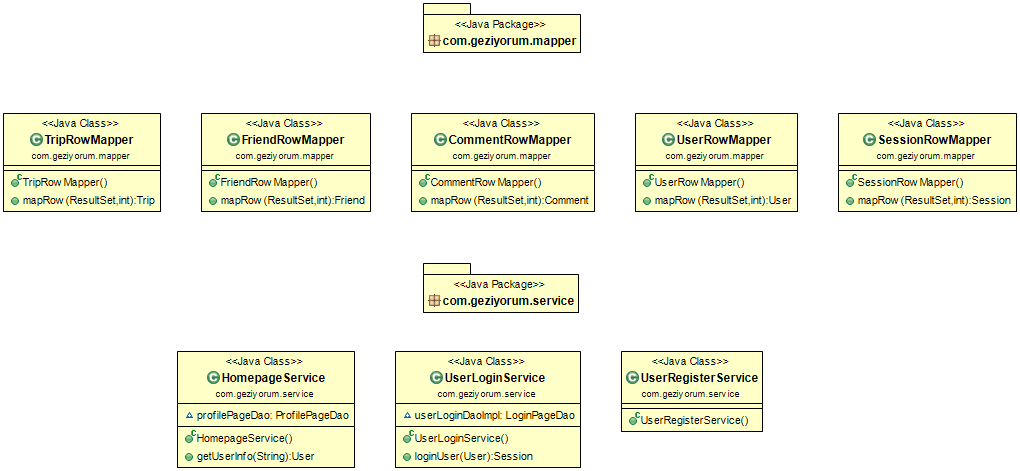
\includegraphics[width=\textwidth]{projectChapters/images/backend3.png}
\caption{Backend implementation MVC UML-3}
\end{figure} 

\begin{figure}[!htbp]
\centering
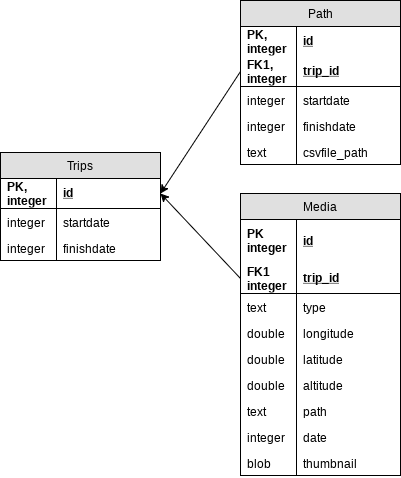
\includegraphics[width=\textwidth]{projectChapters/images/android_database.png}
\caption{Mobile Application Database Diagram}
\end{figure} 